\documentclass[conference]{IEEEtran}
\IEEEoverridecommandlockouts
% The preceding line is only needed to identify funding in the first footnote. If that is unneeded, please comment it out.
\usepackage{cite}
\usepackage{amsmath,amssymb,amsfonts}
\usepackage{algorithmic}
\usepackage{graphicx}
\usepackage{hyperref}
\usepackage{textcomp}
\usepackage{xcolor}
\def\BibTeX{{\rm B\kern-.05em{\sc i\kern-.025em b}\kern-.08em
    T\kern-.1667em\lower.7ex\hbox{E}\kern-.125emX}}

\makeatletter
\newcommand{\linebreakand}{%
  \end{@IEEEauthorhalign}
  \hfill\mbox{}\par
  \mbox{}\hfill\begin{@IEEEauthorhalign}
}
\makeatother

\begin{document}

\title{Maneuvering Machine Learning Algorithms to presage the attacks of \textit{Fusarium oxysporum} on Cotton Leaves\\}

\author{\IEEEauthorblockN{1\textsuperscript{st} Anurag Dutta}
\IEEEauthorblockA{\textit{Department of Computer Science and Engineering} \\
\textit{Government College of Engineering \& Textile Technology}\\
Serampore, Calcutta, India \\
anuragdutta.research@gmail.com}
\and 
\IEEEauthorblockN{2\textsuperscript{nd} Pijush Kanti Kumar}
\IEEEauthorblockA{\textit{Department of Information Technology} \\
\textit{Government College of Engineering \& Textile Technology}\\
Serampore, Calcutta, India \\
pijush752000@yahoo.com}
\linebreakand 
\IEEEauthorblockN{3\textsuperscript{rd} Ankita De}
\IEEEauthorblockA{\textit{Department of Computer Science and Engineering} \\
\textit{Government College of Engineering \& Textile Technology}\\
Serampore, Calcutta, India \\
ankitade2001@gmail.com}
\and 
\IEEEauthorblockN{4\textsuperscript{th} Padmanavan Kumar }
\IEEEauthorblockA{\textit{Department of Computer Science and Engineering} \\
\textit{Kalinga Institute of Industrial Technology}\\
Bhubaneswar, Odisha, India \\
padmanavan2021@gmail.com}
\linebreakand 
\IEEEauthorblockN{5\textsuperscript{th} John Harshith}
\IEEEauthorblockA{\textit{Department of Computer Science and Engineering} \\
\textit{Vellore Institute of Technology University, Vellore Campus}\\
Vellore, Tamil Nadu, India \\
johnharshith@icloud.com}
}

\maketitle

\begin{abstract}
Web technologies have reached unprecedented levels during this time of modernization. Significant and relevant technological stacks like as IoT (Internet of Things), ML (Machine Learning), and AI influenced crawling and cradling (Artificial Intelligence). These categories are really beneficial. In this work, we would try to make use of the notion of Machine Learning Algorithms to predict the attack of \textit{Fusarium oxysporum} on the leaves of the Cotton plant. It's a type of ascomycete fungi that forms an infrageneric grouping called section. All of the species, variations, and forms discovered by Wollenweber and Reinking are Elegans. It belongs to the \textit{Nectriaceae} family. Many strains of the F. oxysporum complex are soil-borne plant pathogens, especially in agricultural settings, despite the fact that their primary function in native soils may be as benign or even advantageous plant endophytes or soil saprophytes. There are many textile products that are made from cotton. Cotton is used in a variety of products besides the textile industry, including gill nets, coffee filters, tarpaulins, cotton paper, and bookbinding. Cotton used to be used to make fire hoses. India and China are the major cotton producers in 2017, with annual production of approximately 18.53 million tonnes and 17.14 million tonnes, respectively. The vast majority of this output is used by their individual textile businesses. This contributes a major portion of the economy. To strengthen the same, we can make use of certain prediction technique that could clearly foresee if the leaves of cotton suffering from the attack by the pathogens, making use of algorithms like 'Support Vector Machine', 'Random Forest', 'k - Nearest Neighbours', and many more. Further this work would also compare the efficacy of these algorithms in predicting the damage in the Cotton Leaves. All Codes, Data, and Supplementary Material are made available at \href{https://github.com/Anurag-Dutta/Maneuvering-Machine-Learning-Algorithms-to-presage-the-attacks-of-Fusarium-oxysporum-on-Cotton-Leave}{https://github.com/Anurag-Dutta/Maneuvering-Machine-Learning-Algorithms-to-presage-the-attacks-of-Fusarium-oxysporum-on-Cotton-Leave}\\
\end{abstract}

\begin{IEEEkeywords}
Machine Learning, Textile Industry, Cotton, Fusarium oxysporum.
\end{IEEEkeywords}
\section{Introduction}
In the Gossypium genus [1] of the Malvaceae family [2] of mallow plants, cotton is a soft, frothy staple fibre that forms a berg, or protective casing, around the seeds. With trace amounts of wax, fat, pectin, and water, cellulose makes up the majority of the fiber's composition. In their natural context, cotton florets will speed up the dispersal of seeds. The shrub-like plant is indigenous to tropical and subtropical areas of the world, including the Americas, Africa, Egypt, and India. The majority of wild cotton varieties are found in Mexico, with Australia and Africa coming in second and third. In order to create a soft, airy, and long-lasting textile, the fibre is most frequently transformed into yarn or thread. It is known that cotton has been used for clothing since the Palaeolithic era [3]. Cotton fabric remnants from the civilization of Indus Valley [4] and Peru dating to 4200 BC have also been discovered. Even though cotton has been grown since ancient times, it wasn't until the cotton gin's invention that the cost of manufacturing was brought down, making cotton the most popular natural fabric for clothing in use today. With 2.5\% of the planet's arable land used, the current estimates for global output are around 110 million bales or 25 million tonnes annually. The biggest manufacturer of cotton in the world is India. For a long time, the top exporter was the United States. The earliest known usage of cotton in the Old World, dating to 5500 BC and preserved in copper beads, was found in the Neolithic settlement of Mehrgarh, which is currently in Balochistan, Pakistan, and is situated at the base of the Bolan Pass. Remains of cotton fabric have been found at Mohenjo-daro [5] as well as other sites, suggesting that cotton may have been a substantial export from the Bronze Age Indus River region. \\

Up till the 19th century, Bengali cotton textiles [6], in particular, continued to hold a competitive advantage. Britain invested in labor-saving technological advancement while enacting protectionist measures like bans and taxes to limit Indian imports in a bid to compete with India. While Bengal was conquered by the East India Company in 1757, the money amassed from Bengal was utilized to put money in British industries like textile production and significantly increase British wealth. During the same period, the East India Company's regulation in India made a significant contribution to its deindustrialization [7], establishing a fresh market for British goods. In addition, British colonisation forced the opening of the humongous Indian market to British products, which could be sold there duty- and tariff-free compared to local Indian manufacturers who paid high taxes. Meanwhile, raw cotton from India was imported duty-free to British factories, which used it to make textiles, offering Britain a stranglehold over India's abundant cotton supply and market. India functioned as a sizable natural monopoly for British produced goods as well as a substantial source of raw materials to British industries. In the 19th century, Britain eventually eclipsed India as the largest producer of cotton textiles worldwide. As in later nineteenth and early twentieth centuries, as EIC expanded in India, the cotton processing industry underwent changes. from concentrating on servicing the British market to providing raw cotton to East Asia. As artisanal textiles lost their competitive edge against industrially produced textiles, Europe began to favour the less expensive long-staple American and Egyptian cottons when selecting its own materials. \\

The blend of organic substances [8], mineral deposits [9], gases, liquids, and living things that makes up soil—also alluded to as earth or dirt—supports life. Some scientific definitions differentiate between soil and dirt by limiting the former term to just displaced soil. Conforming to a theory, soil is created when colloids are flushed downstream after organic matter has collected, depositing concentrations of clay, humus, ferric oxide, carbonate, and gypsum [10]. This layer is known as the B horizon [11]. As sand, silt, clay, and humus mixtures will sustain biologic and agronomic activity prior to the scheduled period, this definition is fairly arbitrary. The movement of these components from one stratum to another is facilitated by animal and water activity. As a result, the soil profile develops horizons. Unique soil horizons are created by the change and movement of elements inside a soil. More modern definitions of soil, however, include non-organic soils like the regoliths [12] which formed on Mars [13] and similar conditions in deserts on Earth. Laterite soil [14], alluvial soil [15], peaty soil, red soil, black soil, mountain soil, desert soil, saline and alkaline soil are the main types of soil in India. The organic and inorganic components of the earth's surface that support plant development are referred to as soil. Soil is formed of a variety of components and slowly changes over time. Minerals and weathered rocks are examples of inorganic, or nonliving, materials. The mechanical or chemical process known as weathering reduces rocks to tiny fragments. When rocks are broken down, organic materials—those generated from living things—combine with them. For instance, when plants and animals pass away and disintegrate, the nutrients in the soil are replenished. Following are the types of soil in India:-
\begin{enumerate}
\item \textit{Alluvial soil}: In India, there is 150 square kilometres of soil, most of it alluvial. In the northern plains and river valleys, it is typical. In peninsular India, they are primarily found in deltas and estuaries. Lime, hummus, and organic materials are all present. The earth here is incredibly fertile. New alluvium is referred to as Khadar, and old alluvium is referred to as Bhangar. The hue of the soil ranges from light grey to ash grey. The Indus-Ganga-Brahmaputra plain [16], the Narmada-Tapi plain [17], and other plains serve as examples.
\item \textit{Red soil}: Usually found in regions with little rainfall, this dirt. The Omnibus group is another name for this soil. Red soil has a pore structure and is friable. The colour is red and the lower layer is yellow or reddish yellow due to the presence of ferric oxide. Red soil is used to grow crops like wheat, cotton, legumes, tobacco, oilseeds, potatoes, and other things.
\item \textit{Regur soil}: The ideal soil for growing cotton is black or regur soil, which is referred to as "regur" in Arabic. The Deccan is mostly covered in black soil. The ability of this soil to retain water is very great. Black dirt has the ability to self-plow and, when dry, forms large fractures. Black soil is a variety of dark to light black in colour and is a good source of iron, lime, calcium, potassium, aluminium, and magnesium.
\item \textit{Desert soil}: The main cause of the deposition of this soil, which is found in dry and semi-arid regions, is wind activity. has a lot of salt in it. Humus and moisture levels in this soil are low. In this soil, kankar is plentiful. The dirt is coloured from red to brown.
\item \textit{Laterite soil}: Brick is the meaning of the Latin term laterite. When wet, this soil is soft; when dry, it becomes hard. The formation of laterite soil, which is found in regions with high temperatures and rains, involves extensive leaching. Since the humus is swiftly absorbed by trees and the organic matter in the soil is quickly destroyed by bacteria owing to the high temperature, this soil's low humus content is one of its key characteristics. Iron and aluminium are abundant in another laterite. Iron oxide is the cause of the soil's red colour. The most widespread crops are cashew nuts, ragi, rice, and sugarcane.
\item \textit{Saline soil}: Saline soil is often referred to as usara soil. Saline soils are referred to locally by the names Reh, Kallar, Chopan, Rakar, Thur, Karl, and so on. These soils formed in regions that had arid weather (with slightly higher rainfall than desert soils) and poor drainage. In this situation, capillary action deposits sodium, calcium, and magnesium salts on the top soil layer. The Southwest Monsoon transports salt flakes and deposits them as a crust in the Rann of Kuchchh. Additionally, in coastal regions, these soils are created when salt water seeps onto the ground during high tide. Furthermore, seawater intrusions in deltas encourage the development of salty soils. In places where it rains a lot and it is humid, marshy soil is present. Here, vegetation grows quite slowly. This soil is alkaline because it has a lot of humus, or dead organic stuff. This soil has a dark colour and a dense texture.
\item \textit{Sub-mountain soil}: This soil is acidic and deficient in humus. The Himalayan areas, Sikkim, Assam, Arunachal Pradesh, and Kashmir, as well as the Peninsula, Eastern Ghats, and Sahyadris summits, are where mountain soils are most prevalent.
\end{enumerate}

Due to the presence of these huge variety of soils in India, India is a leading producer of organic goods in the world. So is the scenario with Cotton. India is it's largest producer. Now, it's obvious that the more we can fetch from these organic products, the more stable, our country's economy would be. We would thus hereby try to safeguard the Cotton Production by identifying potential chances of attack by the pathogens. For that, in this work, we have incorporated the emerging technology in Computer Science - Machine Learning. Normally, it's difficult for farmers to detect the attack of pathogens in the field with naked eyes. But, by making use of Machine Learning techniques, and specifically efficient Machine Learning Algorithms, we would be able to predict the pathogen attacks quite efficiently. For the prediction, we would make use of the prevalent ML Algorithms, like SVM, kNN, Random Forest, etc. 
\section{Cotton Production}
A lengthy frost-free time, lots of sunshine, and a reasonable amount of rainfall—typically between 60 and 120 cm—are necessary for the successful production of cotton. Although the amount of nutrients does not have to be very high, soils often need to be somewhat dense. In both the Northern and Southern hemispheres, these parameters are often satisfied in the seasonally dry tropics and subtropics; nevertheless, a significant amount of the cotton grown today is grown in regions with lower rainfall that receive their water from irrigation. Usually, the crop production for a particular year begins soon after the previous autumn's harvest. Although it is a perennial plant by nature, cotton is produced as an annual to aid with pest management. In the Northern Hemisphere, planting season typically lasts from early February until early June. The greatest continuous cotton-growing region in the world is located in the South Plains region of the United States. Although dryland cotton can be successfully farmed here, the Ogallala Aquifer irrigation water is heavily reliant on for reliable harvests. Cotton is a desirable crop for arid and semiarid environments because it can tolerate some salt and drought. Water-dependent economies confront challenges, conflict, and potential environmental issues as water resources become more scarce globally. Cotton can also be grown to have hues other than the off-yellowish hue that characterises most commercial cotton fibres today. Red, green, and various tones of brown are among the naturally occurring colours of cotton. Cotton fibres have a much bigger water footprint than the majority of other plant fibres. One kilogramme of cotton typically requires between 8,000 and 10,000 litres of water worldwide, and in dry regions like some of India, it may need as much as 22,500 litres. Cotton is also regarded as a thirsty crop. The development of genetically modified cotton aimed to lessen the heavy reliance on pesticides. The Bacillus thuringiensis [18] bacterium naturally creates a chemical that is innocuous to other living forms but damaging to a tiny percentage of insects, most notably the larvae of moths, butterflies, beetles, and flies. Cotton has had the Bt toxin gene introduced into it, resulting in Bt cotton, which produces this organic insecticide in its tissues. Lepidopteran larvae are the primary pests in commercial cotton in many areas, and the Bt protein in the transgenic cotton they consume kills them. This eliminates the need to kill lepidopteran pests by using vast quantities of broad-spectrum insecticides. This helps to manage pests without using insecticides and spares the natural insect predators that are essential to farm ecology. Organic cotton is commonly defined as cotton derived from non-genetically modified plants and produced without the addition of any artificial agricultural agents, such as fertilisers or pesticides. Although a limited number of producers are shifting toward an organic production model, the cotton sector mainly relies on chemicals such as fertilisers, insecticides, and herbicides. Most organic products do not contain transgenic Bt cotton, which includes a bacterium gene that encodes for something like a plant-produced protein that seems to be harmful to a variety of pests, particularly bollworms. Bt cotton has allowed most farmers to significantly reduce their usage of synthetic insecticides, yet resistance may become an issue in the long run. Most cotton is harvested mechanically in the United States, Europe, and Australia, either by a farmhand, a machinery that pulls the cotton off the boll without injuring the cotton crop, or by a cotton extractor, which removes the entire boll from the plant. Cotton strippers are employed in areas in which it is too gusty to grow picker kinds of cotton, usually following the deployment of a pharmaceutical defoliant or natural defoliation caused by a freeze. Cotton is a tropical perennial crop that would continue to grow in the absence of defoliation or frost. The boll weevil has historically been one of the most economically harmful pests in North American cotton production. Boll weevils are bugs that consumed cotton in the 1950s, which significantly decreased the cotton industry's output. A sense of powerlessness was brought on by "this bone pile of tight budgets, market share losses, failing prices, abandoned farms, and the new immunity of boll weevils." Beginning in Beeville, Texas, Boll Weevils decimated cotton fields throughout south Texas. This Boll Weevil swarm devastated everything in its path as it moved from east Texas to the eastern seaboard, forcing many cotton producers out of business.
\section{Dataset}
The Dataset that we are going to make use over here is made avaialable publicly at \href{https://github.com/Anurag-Dutta/Maneuvering-Machine-Learning-Algorithms-to-presage-the-attacks-of-Fusarium-oxysporum-on-Cotton-Leave/tree/main/dataset}{https://github.com/Anurag-Dutta/Maneuvering-Machine-Learning-Algorithms-to-presage-the-attacks-of-Fusarium-oxysporum-on-Cotton-Leave/tree/main/dataset}. The dataset cointains 419 images of both healthy and affected leaves, which have been diviided into 2 parts following the 80 - 20 rule, into test and train data. The images were of different resolutions and had different image parameters. For mitigating these protrusions, we have mapped own each of the images to a fixed resolution of 200 $\times$ 200 pixels, and turning them to gray scale images. This also helped us to get reif of any unnecessary noise in the data. 
\section{Results}
For the prediction, we made use of several Machine Learning Algorithms, namely, 
\begin{enumerate}
\item \textit{Support Vector Machine}: Support vector machines [19] are supervised learning models with a learning algorithm that analyse data for regression and classification in machine learning. Developed by AT\&T Bell Laboratories employees Vladimir Vapnik and others. SVM is one of the most reliable statistical learning-based forecasting techniques. The SVM training algorithm develops a model that allocates new examples to either group and refers to it as a non-probabilistic bipolar linear classifier given a collection of training sample, each of which is designated as corresponding to a specific binary categories. To increase the distance between two categories, SVM translates training samples to space-based points. On the basis of which half of the gap they are on, new samples are then projected to the identical space and anticipated to fit into a particular category. SVMs can effectively do nonlinear classification utilising so-called kernel techniques by implicitly transforming the intake to a high-dimensional feature space, in in addition to linear classification.
\begin{verbatim}
==========================
[ Support Vector Machine ]
==========================

________

TRAINING
________

Training Score: 0.9869646182495344

_______

TESTING
_______

Testing Score: 0.9333333333333333
Precision: 0.9117647058823529
Recall: 0.9538461538461539
\end{verbatim}
Figure 1 shows the precision recall curve, and Figure 2 shows the confusion matrix. 
\begin{figure}[htbp]
\centerline{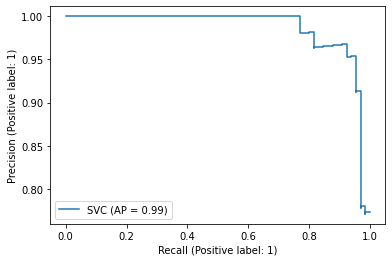
\includegraphics[width = \linewidth]{SVM}}
\label{fig1}
\caption{Graph showing Precision versus Recall for Support Vector Machine}
\end{figure}
\begin{figure}[htbp]
\centerline{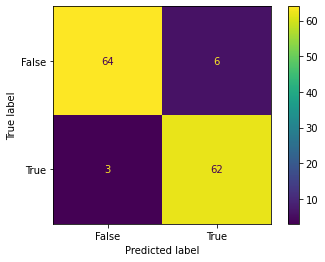
\includegraphics[width = \linewidth]{CM_SVM}}
\label{fig2}
\caption{Confusion Matrix for Support vector Machine}
\end{figure}
\item \textit{Random Forest}: During training, several decision trees are built using the Random Forest [20] (Random Decision Forest) ensemble learning approach, which can be used for classification, regression, and other tasks. A random forest's output for classification problems is the classes that the majority of the trees selected. The mean or mean forecast for each tree is returned for regression tasks. The decision tree's propensity to overfit the training set is corrected by Random Decision Forest. Decision trees are typically outperformed by random forests, however gradient-boosted trees are more accurate. Performance, however, might be impacted by data attributes.
\begin{verbatim}
==========================
[ Random Decision Forest ]
==========================

________

TRAINING
________

Training Score: 1.0

_______

TESTING
_______

Testing Score: 0.8740740740740741
Precision: 0.8333333333333334
Recall: 0.9230769230769231
\end{verbatim}
Figure 3 shows the precision recall curve, and Figure 4 shows the confusion matrix. 
\begin{figure}[htbp]
\centerline{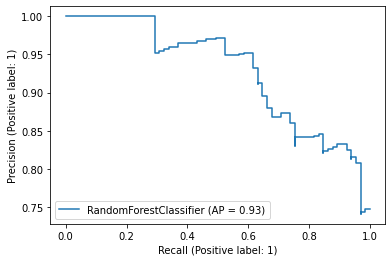
\includegraphics[width = \linewidth]{RF}}
\label{fig3}
\caption{Graph showing Precision versus Recall for Random Decision Forest}
\end{figure}
\begin{figure}[htbp]
\centerline{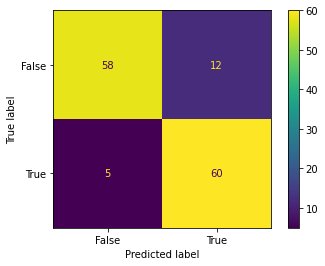
\includegraphics[width = \linewidth]{CM_RF}}
\label{fig4}
\caption{Confusion Matrix for Random Decision Forest}
\end{figure}
\item \textit{k-Nearest Neighbours}: K-Nearest Neighbor [21] is one of the most basic supervised learning-based non-parametric machine learning algorithms. the classification of new instances into categories that are most similar to existing categories, the storage of all pertinent data, and the assumption that new cases and data are comparable to old cases. As a result, using the K-NN approach, it is simple to classify new data into the appropriate categories.
\begin{verbatim}
==========================
[ k - Nearest Neighbours ]
==========================

________

TRAINING
________

Training Score: 0.6108007448789572

_______

TESTING
_______

Testing Score: 0.5703703703703704
Precision: 0.8333333333333334
Recall: 0.9230769230769231
\end{verbatim}
Figure 5 shows the precision recall curve, and Figure 6 shows the confusion matrix. 
\begin{figure}[htbp]
\centerline{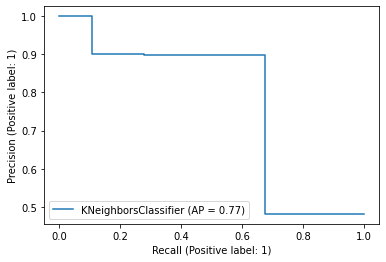
\includegraphics[width = \linewidth]{kNN}}
\label{fig5}
\caption{Graph showing Precision versus Recall for k - Nearest Neighbours}
\end{figure}
\begin{figure}[htbp]
\centerline{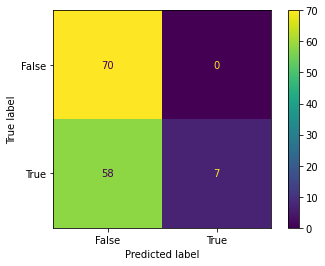
\includegraphics[width = \linewidth]{CM_kNN}}
\label{fig6}
\caption{Confusion Matrix for k - Nearest Neighbours}
\end{figure}
\item \textit{Gaussian Naive Bayes}: It's easy to create classifiers using the Naive Bayes method [22]. A model that selects class labels from a finite set and represents class labels as a vector of feature values gives class labels to problem occurrences. Although there isn't one specific strategy for training these classifiers, there is a series of algorithms built on similar ideas. All naive Bayesian classifiers use the assumption that, given the class variables, the value of a single feature is independent of the value of another feature. For instance, an apple is a round, red fruit with a 10 centimetre diameter. Any potential correlations between the colour, roundness, and diameter variables are also evaluated, as well as the likelihood that the fruit is an apple, by a straightforward Bayesian classifier. Many practical applications employ maximum likelihood techniques for parameter estimation of simple Bayesian models. In other words, simple Bayesian models can be used without adopting or employing Bayesian probability. Despite their basic design and extremely simplified assumptions, naive Bayesian classifiers perform well in a range of difficult real-world circumstances. There are solid theoretical foundations for the ostensibly exceptional performance of straightforward Bayesian classifiers, according to a study of Bayesian classification challenges published in 2004. Bayesian classification, however, triumphs over other strategies like boosted trees and random forests in a comprehensive comparison with other classification methods in 2006. Naive Bayes' benefit is that it just needs a little amount of training data to estimate the classification parameters. 
\begin{verbatim}
=========================
[ Gaussian Naive Bayes  ]
=========================

________

TRAINING
________

Training Score: 0.8100558659217877

_______

TESTING
_______

Testing Score: 0.8074074074074075
Precision: 0.7746478873239436
Recall: 0.8461538461538461
\end{verbatim}
Figure 7 shows the precision recall curve, and Figure 8 shows the confusion matrix. 
\begin{figure}[htbp]
\centerline{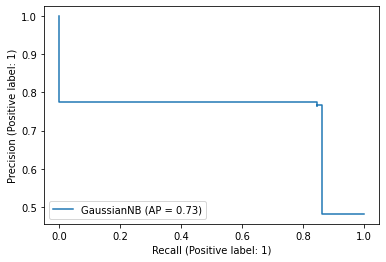
\includegraphics[width = \linewidth]{GNB}}
\label{fig7}
\caption{Graph showing Precision versus Recall for Gaussian Naive Bayes}
\end{figure}
\begin{figure}[htbp]
\centerline{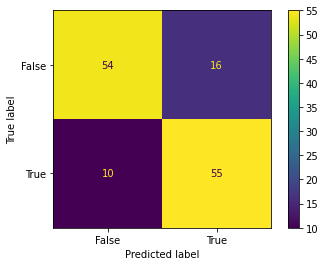
\includegraphics[width = \linewidth]{CM_GNB}}
\label{fig8}
\caption{Confusion Matrix for Gaussian Naive Bayes}
\end{figure}
\item \textit{Logistic Regression}: A logistic model is a statistical model that represents the likelihood of an event occurring by considering the event's log-odds as a linear combination of one or more independent variables. In regression analysis, logistic regression is used to estimate the parameters of a logistic model, which are the coefficients of a linear combination. In binary logistic regression [23], there is a single binomial dependent variable represented by an indicator variable, with the two values labelled '0' and '1', whereas the independent variables are It might be a binomial or continuous variable. Because the associated probability of a value marked '1' can range between 0 and 1, it is marked. The function that translates log odds to probabilities is called a logistic function, thus the name.
\begin{verbatim}
========================
[ Logistic Regression  ]
========================

________

TRAINING
________

Training Score: 1.0

_______

TESTING
_______

Testing Score: 0.8074074074074075
Precision: 0.7746478873239436
Recall: 0.8461538461538461
\end{verbatim}
Figure 9 shows the precision recall curve, and Figure 10 shows the confusion matrix. 
\begin{figure}[htbp]
\centerline{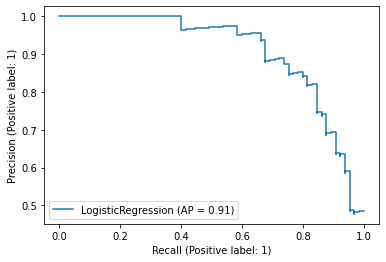
\includegraphics[width = \linewidth]{LR}}
\label{fig9}
\caption{Graph showing Precision versus Recall for Logistic Regression}
\end{figure}
\begin{figure}[htbp]
\centerline{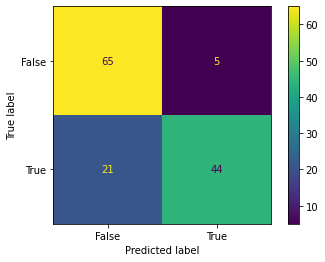
\includegraphics[width = \linewidth]{CM_LR}}
\label{fig10}
\caption{Confusion Matrix for Logistic Regression}
\end{figure}
\end{enumerate}
\section{Conclusion}
Herby, we would like to conclude our work and the discussions thrown about, in the paper. From the results, it's quite clear that the Support Vector Machine Algorithm is best for Predicting the possible attacks of the pathogens in the Cotton Leaves. This Algorithm could be implemented the purpose to cater well with high performance. Further, the work in our paper could be extended by making use of newer and better algorithm for Prediction. Certain Artificial Neural Networks, like ChaosNet could also be used. ChaosNet, being an ANN built of 1 - D Generalized Luroth Series, is given the ability to perform supervised learning by taking only a few data points for training. The same notion can be applied for other plant diseases, and which in turn could help us in gaining a better ecological balance with the nature, which would also benefit us socially, and economically. 
\begin{thebibliography}{00}
\bibitem{b1} M. Wang et al., “Genomic innovation and regulatory rewiring during evolution of the cotton genus Gossypium,” Nature Genetics, vol. 54, no. 12, pp. 1959–1971, Dec. 2022, doi: 10.1038/s41588-022-01237-2.
\bibitem{b2} G. Albani Rocchetti et al., “Selecting the best candidates for resurrecting extinct-in-the-wild plants from herbaria,” Nature Plants, vol. 8, no. 12, pp. 1385–1393, Dec. 2022, doi: 10.1038/s41477-022-01296-7.
\bibitem{b3} C. Conneller, “The view at the end of the Palaeolithic world,” Nature Ecology \& Evolution, vol. 6, no. 11, pp. 1591–1592, Oct. 2022, doi: 10.1038/s41559-022-01899-5.
\bibitem{b4} S. A. Romshoo, K. O. Murtaza, and T. Abdullah, “Towards understanding various influences on mass balance of the Hoksar Glacier in the Upper Indus Basin using observations,” Scientific Reports, vol. 12, no. 1, Sep. 2022, doi: 10.1038/s41598-022-20033-w.
\bibitem{b5} B. Ansumali Mukhopadhyay, “Ancestral Dravidian languages in Indus Civilization: ultraconserved Dravidian tooth-word reveals deep linguistic ancestry and supports genetics,” Humanities and Social Sciences Communications, vol. 8, no. 1, Aug. 2021, doi: 10.1057/s41599-021-00868-w.
\bibitem{b6} M.-H. Gao et al., “Himalayan zircons resurface in Sumatran arc volcanoes through sediment recycling,” Communications Earth \& Environment, vol. 3, no. 1, Nov. 2022, doi: 10.1038/s43247-022-00611-6.
\bibitem{b7} A. Shkembi, L. M. Smith, and R. L. Neitzel, “Linking environmental injustices in Detroit, MI to institutional racial segregation through historical federal redlining,” Journal of Exposure Science \& Environmental Epidemiology, Dec. 2022, doi: 10.1038/s41370-022-00512-y.
\bibitem{b8} E. P. Suosaari et al., “Authigenic clays as precursors to carbonate precipitation in saline lakes of Salar de Llamara, Northern Chile,” Communications Earth \& Environment, vol. 3, no. 1, Dec. 2022, doi: 10.1038/s43247-022-00658-5.
\bibitem{b9} G. L. Walters, S. J. Kemp, J. D. Hemingway, D. T. Johnston, and D. A. Hodell, “Clay hydroxyl isotopes show an enhanced hydrologic cycle during the Paleocene-Eocene Thermal Maximum,” Nature Communications, vol. 13, no. 1, Dec. 2022, doi: 10.1038/s41467-022-35545-2.
\bibitem{b10} Y. Zhou, X. Li, Y. Shi, Q. Zhu, and J. Du, “Reuse of phosphogypsum pretreated with water washing as aggregate for cemented backfill,” Scientific Reports, vol. 12, no. 1, p. 16091, Sep. 2022, doi: 10.1038/s41598-022-20318-0.
\bibitem{b11} Y. Steinberger et al., “A sensitive soil biological indicator to changes in land-use in regions with Mediterranean climate,” Scientific Reports, vol. 12, no. 1, Dec. 2022, doi: 10.1038/s41598-022-26240-9.
\bibitem{b12} “PLANETARY SCIENCE: Dark Asteroids and Regoliths,” Nature Physical Science, vol. 244, no. 131, pp. 1–1, Jul. 1973, doi: 10.1038/physci244001c0.
\bibitem{b13} V. L. Hartwick, O. B. Toon, J. K. Lundquist, O. A. Pierpaoli, and M. A. Kahre, “Assessment of wind energy resource potential for future human missions to Mars,” Nature Astronomy, Dec. 2022, doi: 10.1038/s41550-022-01851-4.
\bibitem{b14} J. Zheng, Z. Yang, H. Gao, X. Lai, X. Wu, and Y. Huang, “Experimental study on microstructure characteristics of saturated remolded cohesive soil during consolidation,” Scientific Reports, vol. 12, no. 1, Nov. 2022, doi: 10.1038/s41598-022-23323-5.
\bibitem{b15} A. D’Agostino et al., “Neolithic dental calculi provide evidence for environmental proxies and consumption of wild edible fruits and herbs in central Apennines,” Communications Biology, vol. 5, no. 1, Dec. 2022, doi: 10.1038/s42003-022-04354-0.
\bibitem{b16} S. J. P. Lenard, J. Lavé, C. France-Lanord, G. Aumaître, D. L. Bourlès, and K. Keddadouche, “Steady erosion rates in the Himalayas through late Cenozoic climatic changes,” Nature Geoscience, vol. 13, no. 6, pp. 448–452, Jun. 2020, doi: 10.1038/s41561-020-0585-2.
\bibitem{b17} S. Rawat, A. Ganapathy, and A. Agarwal, “Drought characterization over Indian sub-continent using GRACE-based indices,” Scientific Reports, vol. 12, no. 1, Sep. 2022, doi: 10.1038/s41598-022-18511-2.
\bibitem{b18} E. Sanniyasi, A. P. R. Patrick, K. Rajagopalan, R. K. Gopal, and R. Damodharan, “Characterization and in vitro anticancer potential of exopolysaccharide extracted from a freshwater diatom Nitzschia palea (Kütz.) W.Sm. 1856,” Scientific Reports, vol. 12, no. 1, Dec. 2022, doi: 10.1038/s41598-022-24662-z.
\bibitem{b19} M. S. Mirza, S. M. Munaf, F. Azim, S. Ali, and S. J. Khan, “Vision-based Pakistani sign language recognition using bag-of-words and support vector machines,” Scientific Reports, vol. 12, no. 1, Dec. 2022, doi: 10.1038/s41598-022-15864-6.
\bibitem{b20} K. L. Bacon et al., “Relation of gait measures with mild unilateral knee pain during walking using machine learning,” Scientific Reports, vol. 12, no. 1, Dec. 2022, doi: 10.1038/s41598-022-21142-2.
\bibitem{b21} E. Dann, N. C. Henderson, S. A. Teichmann, M. D. Morgan, and J. C. Marioni, “Differential abundance testing on single-cell data using k-nearest neighbor graphs,” Nature Biotechnology, vol. 40, no. 2, pp. 245–253, Sep. 2021, doi: 10.1038/s41587-021-01033-z.
\bibitem{b22} H. Pan, S. He, T. Zhang, S. Song, and K. Wang, “Application of an improved naive Bayesian analysis for the identification of air leaks in boreholes in coal mines,” Scientific Reports, vol. 12, no. 1, Sep. 2022, doi: 10.1038/s41598-022-20504-0.
\bibitem{b23} Y. Liu, C. Xu, C. Xing, and M. Chen, “Influencing factors and prediction methods of radiotherapy and chemotherapy in patients with lung cancer based on logistic regression analysis,” Scientific Reports, vol. 12, no. 1, Dec. 2022, doi: 10.1038/s41598-022-25592-6.
\end{thebibliography}
\end{document}
